% Template for a Thesis
%
% 7-results.tex
%
% Results

\chapter{Results}\label{ch:results}

This chapter shows the results and analysis for each step of the development of this thesis, ranging from score plots for BPE alignments, to algorithm runtimes. The scores display four different metrics, namely precision, recall, F1 score and AER, which have been explained previously in the Translation chapter.~\ref{tra:metrics}

\section{Replication of BPE}

When replicating BPE, the best BPE result using \emph{Fastalign} as alignment algorithm is a F1 score of 0.609, obtained after 1000 BPE merges. The baseline has a F1 score of 0.6. Baseline in this situation refers to the scores when aligning the raw corpus, leaving the words untouched and with no BPE units.

\begin{figure}[!ht]
    \centering
    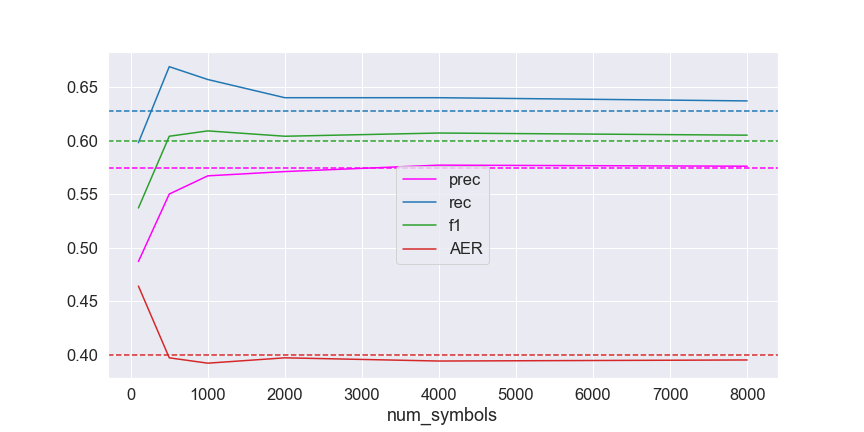
\includegraphics[width=13cm]{../reports/scores_normal_bpe/eng_deu_fastalign.png}
    \caption{Scores of BPE over baseline, using Fastalign}
\end{figure}

In the case of \emph{Eflomal}, the baseline F1 score is 0.72, and the best F1 score is 0.701, obtained after 6000 merges. When using \emph{Eflomal}, BPE does not improve the baseline.

\begin{figure}[!ht]
    \centering
    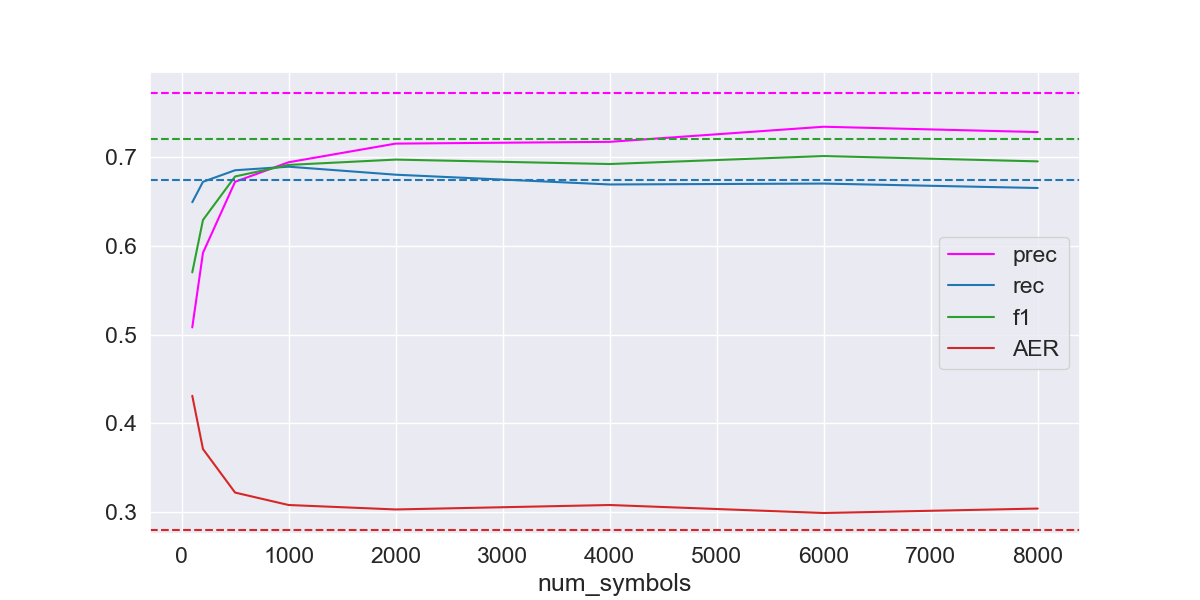
\includegraphics[width=13cm]{../reports/scores_normal_bpe/eng_deu_eflomal.png}
    \caption{Scores of BPE over baseline, using Eflomal}
\end{figure}

The alignment algorithms, \emph{Fastalign} and \emph{Eflomal}, require one language to be given as source and the other as target, and perform the alignment based on this. Throughout the thesis, English has been taken as the source language and German as the target. It might have been interesting to see that swapping the languages would yield different results, by swapping the languages in the global variables file. The difference between these two cases is barely perceptible, a difference of 0.03\% throughout the scores across all numbers of merges. Therefore, it is assumed that swapping the source and target language has no effect in the experiment result scores.

\section{Replication of BPE-dropout}

BPE-dropout is meant to be an improvement of BPE, therefore the desired score comparison is that of BPE-dropout with respect to BPE. The BPE scores are taken as baseline, instead of the gold standard scores as in the previous case. As explained in the Methodology chapter~\ref{met:replbpedrop}, the BPE dropout pipeline is run a number of times, resulting in many possible segmentations. Out of these, three types of results are obtained: union, intersection and threshold.

\begin{itemize}
	\item The \textbf{union} case takes all alignments into account, resulting in a big list of alignments per sentence. These most probably include the correct alignments, but there are many other wrong alignments. This case has low precision and high recall.
	\item The \textbf{intersection} case takes only those alignments which are present in all alignment files, resulting in a few number of alignments per sentence. Most probably, these alignments are correct, but there are also be many alignments missing. This case has high precision and low recall.
	\item The \textbf{threshold} case is a mixture between union and intersection. Given a threshold, for instance 0.7, an alignment is accepted if it is present in 70\% of the alignment files. Smaller values for this variable resemble the union case, since more alignments are accepted. Higher threshold numbers resemble the intersection case, where alignments must be present in more and more files in order to be accepted.
\end{itemize}

The following figures 6.3, 6.4 and 6.5. show the results for a \emph{dropout} rate of 10\%, and the union, intersection and threshold cases.

 \begin{figure}[!ht]
     \centering
     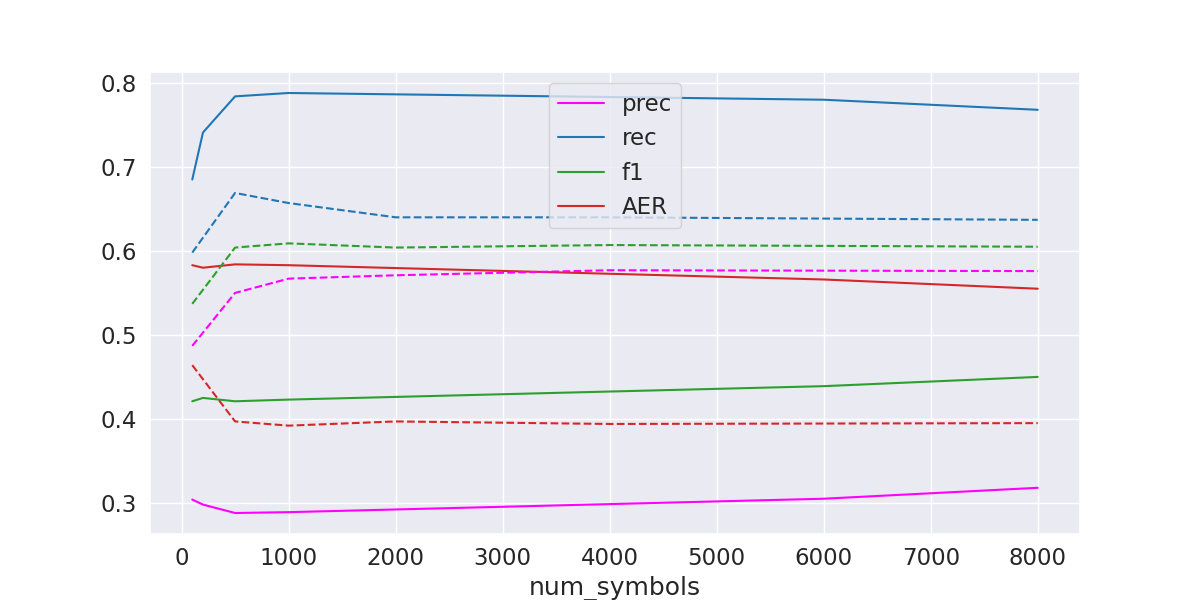
\includegraphics[width=13cm]{../reports/scores_dropout_bpe/space/0.1/eng_deu_union_fastalign.png}
     \caption{Scores for BPE-dropout with dropout rate 0.1, union mode}
 \end{figure}
 
 \begin{figure}[!ht]
     \centering
     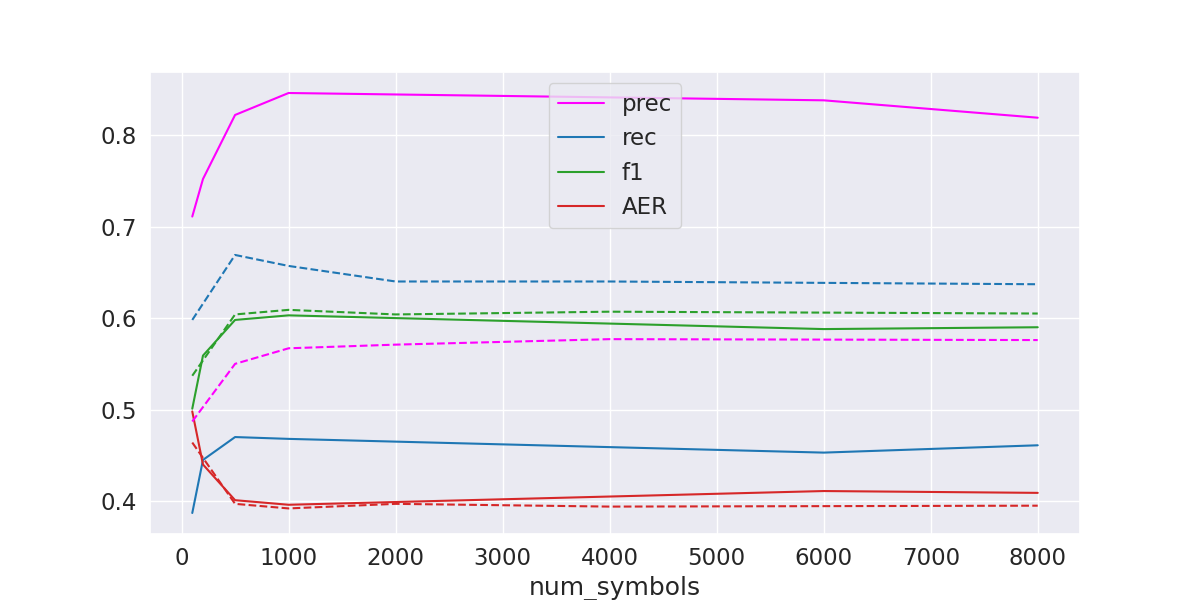
\includegraphics[width=13cm]{../reports/scores_dropout_bpe/space/0.1/eng_deu_inter_fastalign.png}
     \caption{Scores for BPE-dropout with dropout rate 0.1, intersection mode}
 \end{figure}

It can be seen that the F1 score improves consistently the more BPE units have been merged. Since there are more merges, there are fewer units, most words are completely merged and the uncertainty of aligning BPE units is lower, since the sentence looks more and more similar to the raw sentence where there are just words. Regarding the threshold case, the following two figures show the scores for threshold 0.3 and 0.7, \textbf{which achieves the best F1 score, namely 0.635}.

\begin{figure}[!ht]
    \centering
    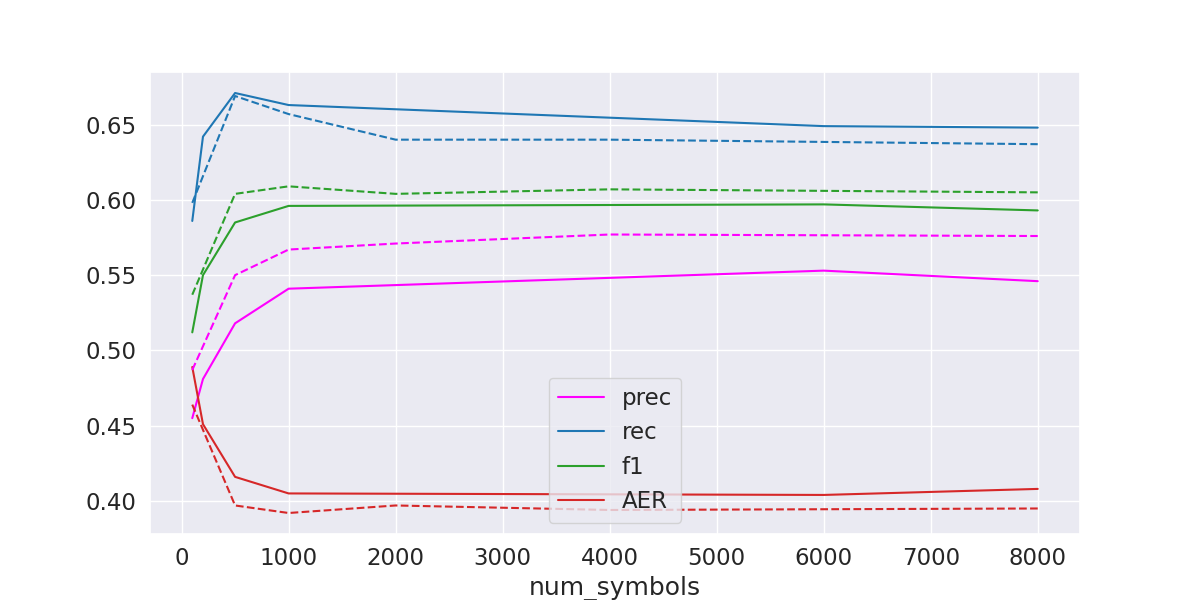
\includegraphics[width=13cm]{../reports/scores_dropout_bpe/space/0.1/eng_deu_0.3_thres_fastalign.png}
    \caption{Scores for BPE-dropout with dropout rate 0.1, threshold mode at 0.3}
\end{figure}

\begin{figure}[!ht]
    \centering
    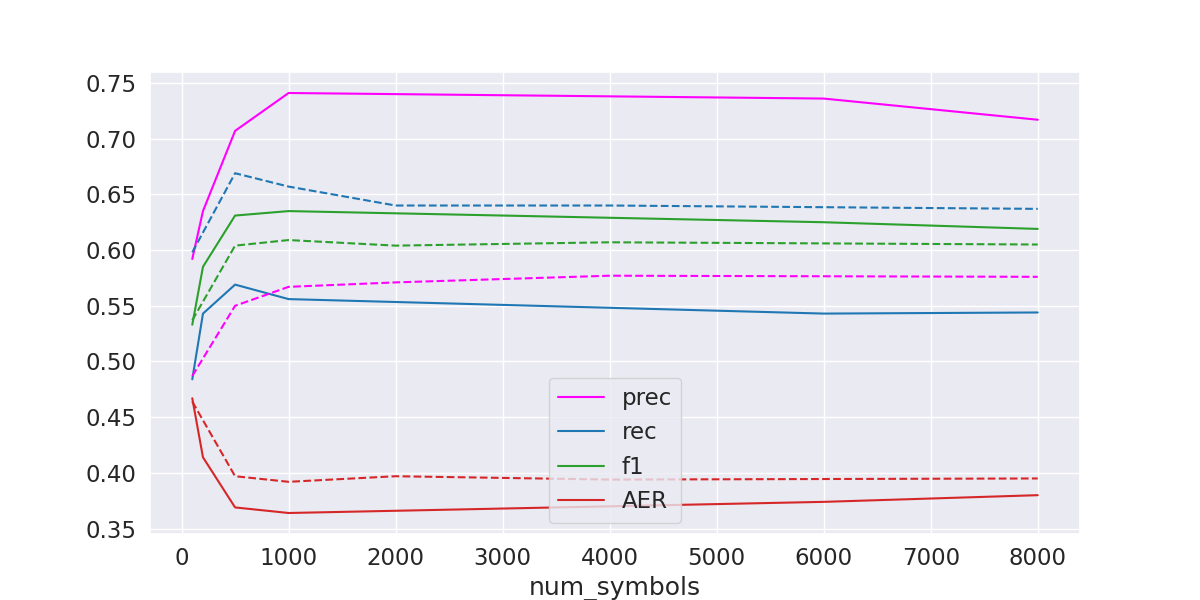
\includegraphics[width=13cm]{../reports/scores_dropout_bpe/space/0.1/eng_deu_0.7_thres_fastalign.png}
    \caption{Scores for BPE-dropout with dropout rate 0.1, threshold mode at 0.7}
\end{figure}

It is visible that the scores plot with the threshold at 0.3 resembles the union case more, and recall goes lower while the precision goes higher for larger threshold values. The optimal result is found at the threshold value of 0.7. This result is replicated when increasing the dropout rate up to 20\% as well as 30\%, and setting the alignment threshold at 0.5. \textbf{This shows that BPEs are robust to dropout}.

In the BPE dropout paper~\cite{provilkov2019bpedropout}, the authors only use one dropout percentage, namely 10\% for all languages and 60\% specifically for Chinese and Japanese to match the increase in length of segmented sentences for other languages. The paper hypothesizes that exposing a model to different segmentations might result in better understanding of the whole words as well as their subword units, which is proven by the paper and by this thesis as well. The paper authors also speculate the following:

\begin{quote}
	Results indicate that using BPE-Dropout on the source side is more beneficial than using it on the target side. We speculate it is more important for the model to understand a source sentence, than being exposed to different ways to generate the same target sentence.
\end{quote}

This theory is also confirmed in this thesis. As the experiment of only applying BPE in English in the English-German language pair shown in the Figure 6.7, the improvement of BPE-dropout over BPE in this case is 3\%.

\begin{figure}[!ht]
    \centering
    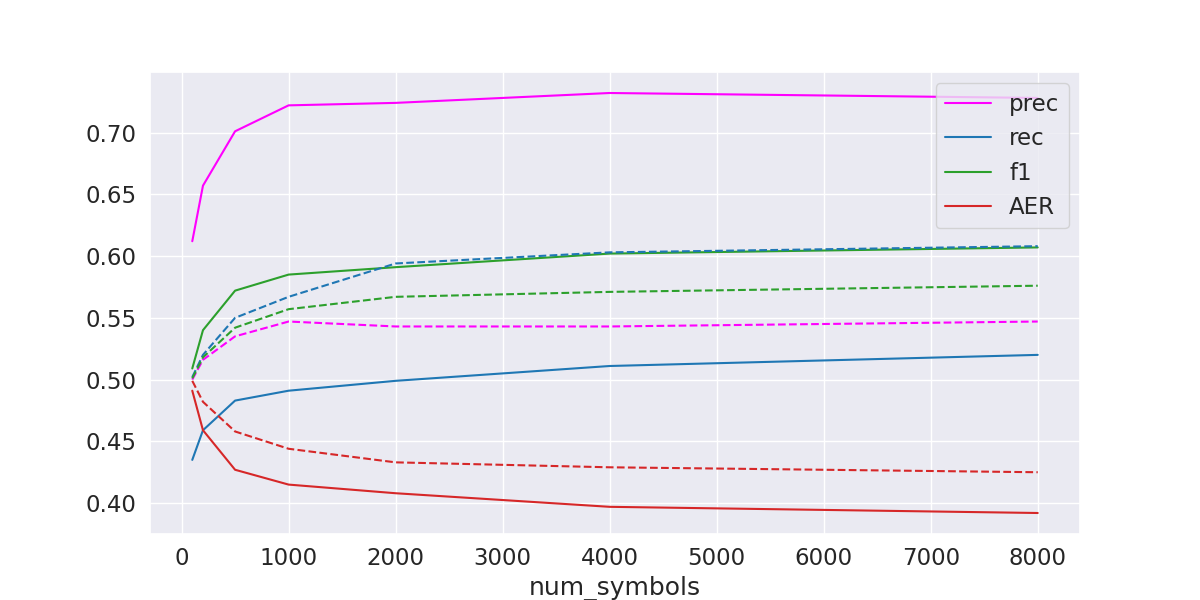
\includegraphics[width=13cm]{../reports/scores_dropout_bpe/space/0.1/eng_deu_0.7_thres_fastalign_eng.png}
    \caption{Scores for BPE-dropout with dropout rate 0.1, threshold at 0.7 and BPE only in source language}
\end{figure}

Regarding the improvements of BPE dropout over normal BPE, the authors conclude the following:

\begin{quote}
	The improvement with respect to normal BPE are consistent no matter the vocabulary size. But we see that the effect from using BPE-Dropout vanishes when a corpora size gets bigger.
\end{quote}

This thesis has predominantly been run with a fixed size, relatively small corpus consisting of 10.000 sentences, whereas the paper authors have used much bigger corpora ranging from 133.000 sentences up to 2 million. As a result, the effect of varying corpus size has not been replicated. However, it can be seen that for bigger number of merges, the effects of BPE dropout are smaller, since given the bigger number of merges, the segmentations resemble the case where no dropout is applied.

As the BPE dropout paper states, \emph{BPE dropout improves BPE consistently no matter how many merges are performed}. This result is replicated in this paper. Additionally, in the paper they use a fixed dropout rate and they give no information as per the threshold used in determining how to aggregate alignments. \textbf{By experimenting with different dropout and threshold rates, it was possible to improve the F1 score by selecting a dropout rate of 30\%, which is specific to the corpus, in this case English and German, creating 30 segmentations and selecting an alignment threshold of 0.5. This results in a F1 score of 0.685, an improvement of 2\% from the previous case}.

\section{BPE-dropout for other language pairs}

The better results of BPE-dropout over BPE proves that BPE-dropout performs better than BPE, at least in the English-German case, and the optimal hyperparameters for this case were using a dropout rate of 10\%, an alignment threshold of 0.7, and around 2000 merges. The 2000 merge hyperparameter might be dependent on the corpus, smaller corpora might not even have 2000 merges to make, while bigger corpora might obtain their optimal results for more merges. \textbf{But does BPE-dropout outperform BPE for other language pairs at a dropout rate of 10\% and an alignment threshold of 0.7?}

A couple of other language pairs were tested, namely English-Romanian, consisting of 50.000 sentences, and English-Hindi, with 3.000 sentences. Merge lists were created for English, Romanian and Hindi, each according to the particular case. For instance, the English merge list in the English-Romanian case is much richer than the merge list in the English-Hindi case, because the former has a much bigger corpus from which to learn frequent sequence pairs. Instead of using the rich English merge list obtained from the 50.000 sentences and applying it to all language pairs, namely German, Romanian and Hindi, it was decided that each language pair would see its own merge list created from the available corpus. The Romanian case, being the corpus around 16 times bigger, takes longer to compute segmentations and alignments but the results are consistent. \textbf{BPE-dropout outperforms BPE in two other language pairs for a dropout rate of 10\%, an alignment threshold of 0.7 and with vastly different corpus sizes}. The BPE-dropout scores are shown in the following figures, the F1 score improvement over BPE for English-Romanian is of 1.5\%, obtained at 4000 merges, and the F1 score improvement over BPE for English-Hindi is of 2.8\%. It is worth noting that given the small size of the English-Hindi corpora, the merge list is only around 5000 merges long.

\begin{figure}[!ht]
    \centering
    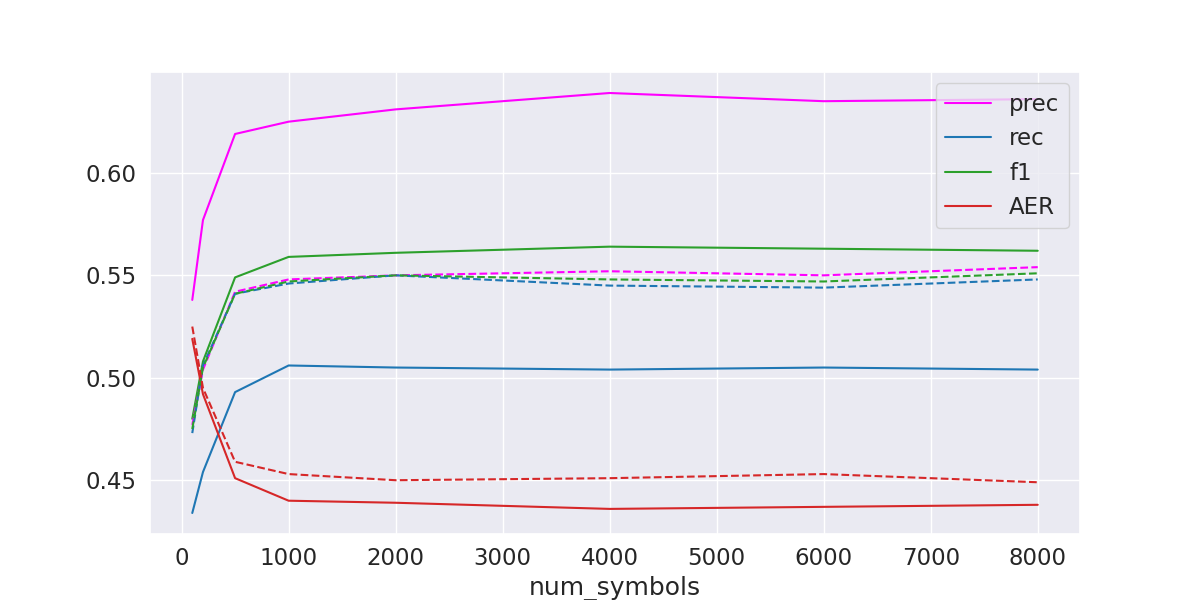
\includegraphics[width=13cm]{../reports/scores_dropout_bpe/space/0.1/eng_ron_0.7_thres_fastalign.png}
    \caption{Scores for BPE-dropout on English-Romanian with dropout rate 0.1, threshold at 0.7}
\end{figure}

\begin{figure}[!ht]
    \centering
    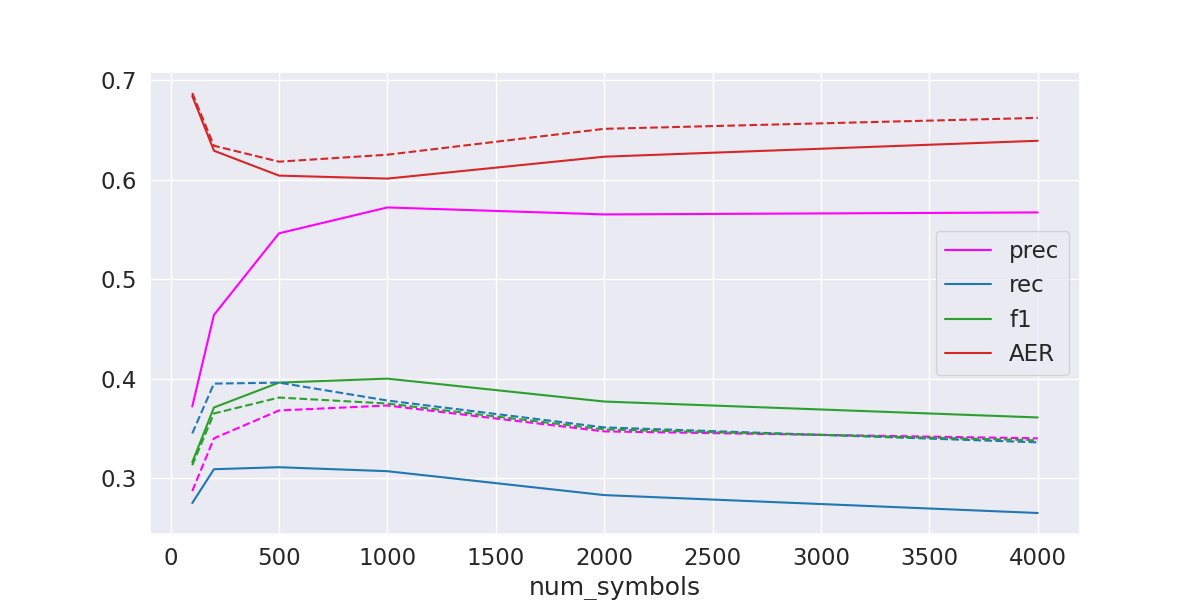
\includegraphics[width=13cm]{../reports/scores_dropout_bpe/space/0.1/eng_hin_0.7_thres_fastalign.png}
    \caption{Scores for BPE-dropout on English-Hindi with dropout rate 0.1, threshold at 0.7}
\end{figure}

\section{Improvement of the learn-BPE algorithm}

By modifying the algorithm to update the corpus after a merge, by introducing indexes and frequency counts to reduce iteration, the learn-BPE algorithm's runtime was dramatically accelerated. In the beginning, the algorithm starts by creating around 1.5 BPE merges per second, which is relatively slow because since the most frequent pairs are so frequent, most of the indexes in the corpus are visited and many update operations are done. The further down in the iterations, the less frequent merges are, the faster it is to merge them and update the corpus. The speed of merges per second gets faster and faster until by the time it is finished with the corpus, it is running at roughly 300 merges per second for English and 120 merges per second in German.

After the improvement, the algorithm, on average, needs \textbf{55s to learn BPE merges in English, and 1:25min in German on corpora composed of 10.000 sentences}. The time difference between English and German is due to the fact that the words in German are generally lower, with a higher variance, and there are therefore more merge possibilities. In contrast, Sennrich et al.~\cite{sennrich2015neural}'s algorithm needs 2:15min for English and 3:20min for German. The algorithm presented here shows an improvement in speed of 2.5x for English and 2.4x for German. These tests have been performed on an Intel Core i5-7200U CPU at 2.5GHz, a 64-bit Windows OS with 8GB RAM.

A C++ implementation of the BPE algorithm from Sennrich et al. can be found on \href{https://github.com/glample/fastBPE}{Github} This package makes use of C++'s advantage to handle memory better than Python, for instance by memory mapping the input file to read it efficiently, and by using multi-threading to pre-compute the BPE splits of all words in the input file. When applied to this thesis' dataset, it barely needs a few seconds to learn BPE codes, making it much faster than the algorithm developed in this thesis. However, this package does not include BPE-dropout or any other word separation rather than \emph{</w>} at the end of the word; it is not possible to create BPE tokens without word boundaries using this method. It is assumed that it would not be very complicated to integrate these two aspects into the package, but given that this algorithm was created by a PhD student, there are no guarantees of maintenance in the future. In contrast, this thesis' algorithm takes more time but depending on \emph{dropout} and \emph{space} parameters, the algorithm is adapted to both scenarios.

\section{No-space results}

Learning BPE units that can handle merges among words takes more time, since there are more possibilities to merge; each end of the word and each beginning of the word can now be merged. In the previous case, there was only a fixed number of merges that could be done inside a word, once the whole word was merged into one unit, no other merges were possible. Now however, that word can be merged with its previous or subsequent tokens.

As with the space case, the algorithm starts relatively slow, at around 0.7 BPE merges per second. While the most frequent merge in the space case is \emph{\_t, h} for English and \emph{e, n} for German, in the no-space case the most frequent merges are \emph{e, \_} for English and \emph{e, n} again for German. In the English case, the pair \emph{e, \_} is much more frequent than the pair \emph{\_t, h}, and it takes more time for this pair to get merged. Afterwards, the number of merges per second increases until plateauing at 50 merges per second in English, and slightly lower in German. The runtime is \textbf{3:50min for 10.000 merges in English and 4:10min in German}. Since there are more merge possibilities, the algorithm was also run \textbf{for 20.000 merges, with a runtime of 9:30min in English and 10min in German}.

Further down the pipeline, alignments are performed without any notion of what words are, and \emph{Fastalign} and \emph{Eflomal} are not thought to handle multiword-to-multiword alignments. It is therefore expected that the scores will be lower than in the space case, and it is also expected that the more BPE merges, the bigger the segmentations, the more words will be merged together. For instance, if the multiword unit \emph{in\_the\_street} is aligned to \emph{auf\_der\_Strasse}, the following mapping would be performed: \emph{in-auf}, \emph{in-der}, \emph{in-Strasse}, \emph{the-auf}, \emph{the-der} and so on. This brings the precision down dramatically, since most of these alignments are incorrect. For the case of no dropout, the best result for BPE without space separations is a F1 score of 0.477, obtained at 200 merges, which is a very low number of merges compared to the previous best scores. The F1 score is also poor relative to the case where merges between words are no allowed. Regardless, given that there is no notion as to what a word constitutes, this result cannot be poorly regarded.

\begin{figure}[!ht]
    \centering
    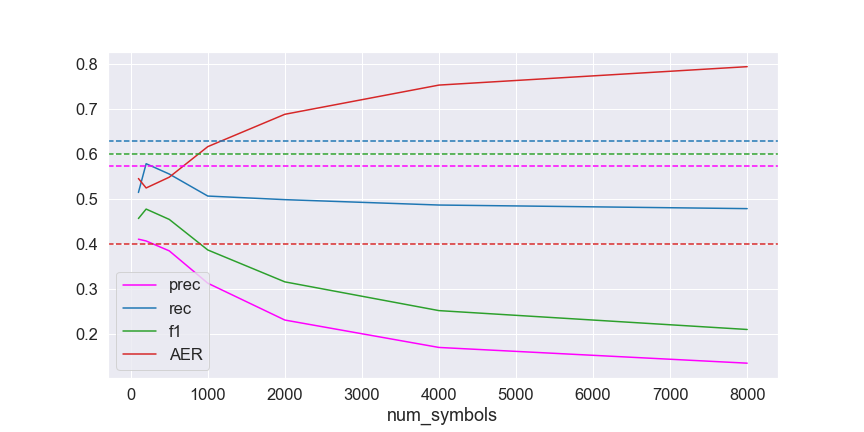
\includegraphics[width=13cm]{../reports/scores_normal_bpe/eng_deu_ns_fastalign.png}
    \caption{Scores for no-space BPE}
\end{figure}

As the following figures show, BPE-dropout outperforms BPE also in no-space mode, making this improvement consistent regardless if word boundaries are considered or not. It can be therefore concluded, that \textbf{BPE-dropout outperforms BPE in all experiments done in this thesis, with word boundaries or without}. For a dropout rate of 10\%, results already improve wtih an F1 score of 0.523 for 200 merges and an alignment threshold of 0.7. The maximum F1 score is obtained at a dropout rate of 20\%, with an \textbf{F1 score of 0.559 for 500 merges and an alignment threshold of 0.5}, which constitutes an improvement of 10.5\% with respect to no-space BPE with no dropout.

\begin{figure}[!ht]
    \centering
    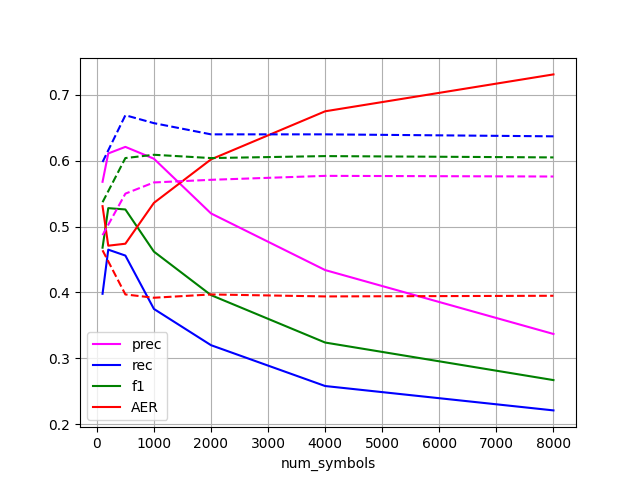
\includegraphics[width=13cm]{../reports/scores_dropout_bpe/no space/0.1/scores_ns_0.7_thres.png}
    \caption{Scores for no-space BPE-dropout with dropout rate 0.1, threshold at 0.7}
\end{figure}

\begin{figure}[!ht]
    \centering
    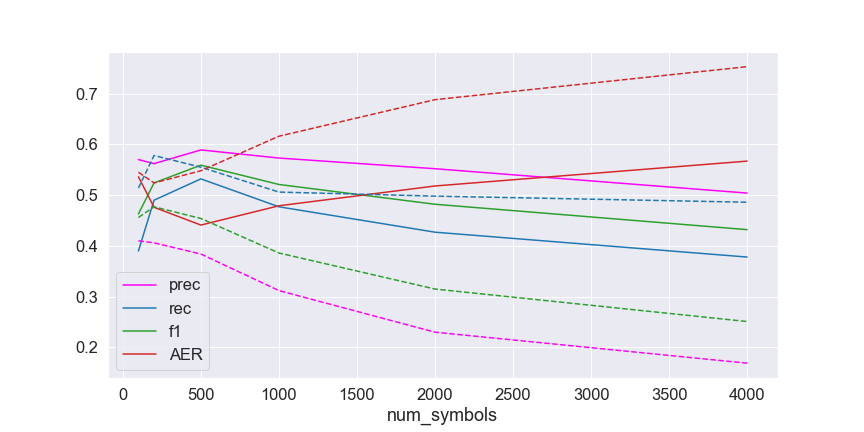
\includegraphics[width=13cm]{../reports/scores_dropout_bpe/no space/0.2/eng_deu_ns_0.5_thres.png}
    \caption{Scores for no-space BPE-dropout with dropout rate 0.2, threshold at 0.5}
\end{figure}

Experiments with higher dropout rates have also been conducted, namely a dropout rate of 50\% which is very large, half the merges are dropped, with a F1 score of 0.529 for 4000 merges and an alignment threshold of 0.3. These parameters are considerably different than the ones previously. The ideal score happens at 4000 merges, which makes sense that it is a bigger number since so many merges are dropped. And the alignment threshold is also very low compared to previous cases, meaning that most alignments are accepted creating a sort of union.

\begin{figure}[!ht]
    \centering
    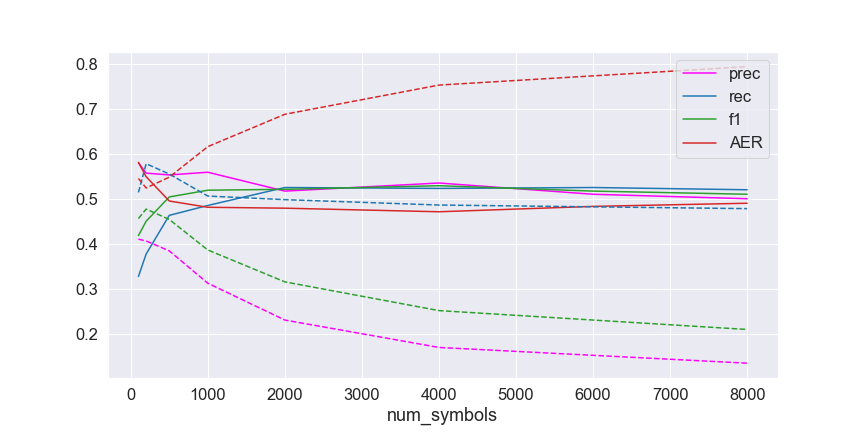
\includegraphics[width=13cm]{../reports/scores_dropout_bpe/no space/0.5/scores_ns_0.3_thres.png}
    \caption{Scores for no-space BPE-dropout with dropout rate 0.5, threshold at 0.3}
\end{figure}

\section{No-space results for other language pairs}

Similarly to the case of BPE-dropout in space mode, where it was shown that BPE-dropout outperforms BPE with a dropout rate of 10\% and an alignment threshold of 0.7, it is also interesting to see the performance of BPE-dropout in no-space mode in other language pairs, in this case with the optimal hyperparameters of no-space mode, namely a dropout rate of 20\% and an alignment threshold of 0.5. The following figures show the performance of BPE-dropout given the baseline of BPE in no-space mode, for the language pairs English-Romanian and English-Hindi. At the ideal hyperparameter of 500 merges, the F1 score improvement of BPE-dropout over BPE in English-Hindi is of 6.2\%, and 8.4\% in English-Romanian.

\begin{figure}[!ht]
    \centering
    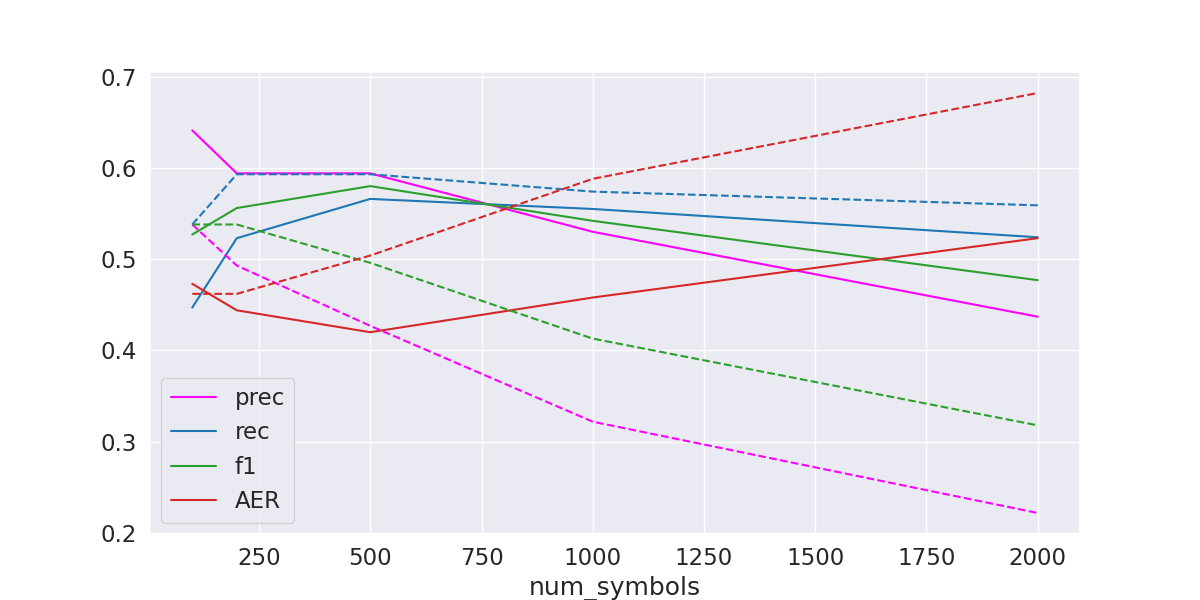
\includegraphics[width=13cm]{../reports/scores_dropout_bpe/no space/0.2/eng_ron_ns_0.5_thres_fastalign.png}
    \caption{Scores for no-space BPE-dropout on English-Romanian with dropout rate 0.2, threshold at 0.5}
\end{figure}

\clearpage
\begin{figure}[!ht]
    \centering
    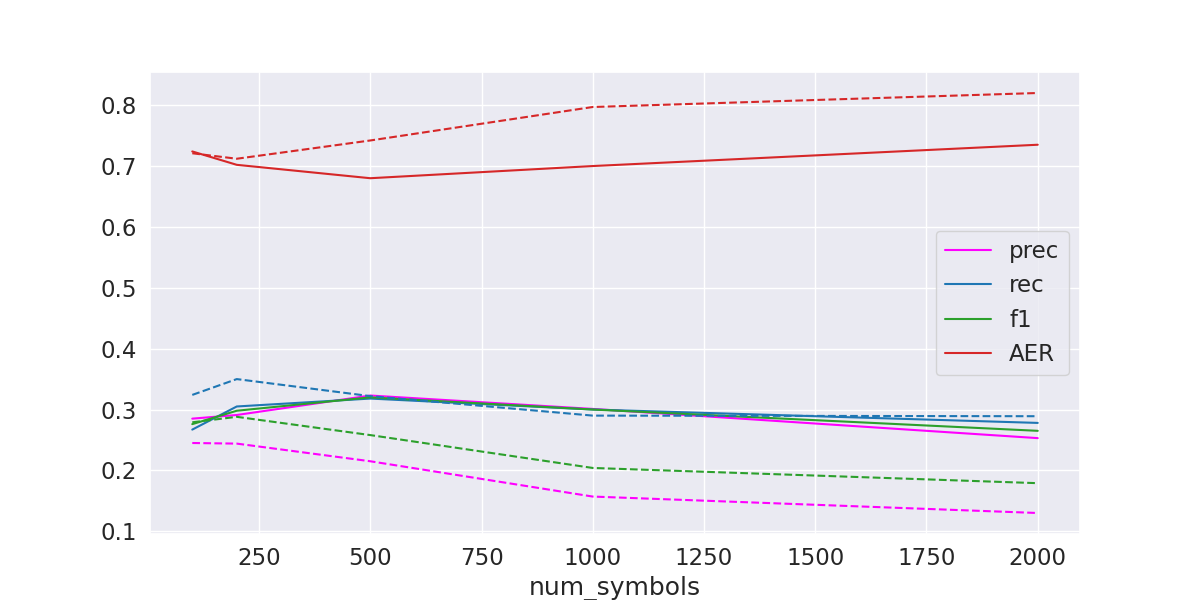
\includegraphics[width=13cm]{../reports/scores_dropout_bpe/no space/0.2/eng_hin_ns_0.5_thres_fastalign.png}
    \caption{Scores for no-space BPE-dropout on English-Hindi with dropout rate 0.2, threshold at 0.5}
\end{figure}

\section{Summary}

The F1 score results of this thesis are summarized as follows:

\begin{quote}
    Eng-Deu word alignment score: 0.6\\
    Eng-Deu BPE score: 0.609\\
    Eng-Deu BPE score, BPE only in Eng: 0.56\\
    Eng-Deu BPE-dropout score: 0.635
\end{quote}

The best hyperparameters for Eng-Deu BPE-dropout are: dropout rate 10\%, 2000 merges, alignment threshold 0.7, 10 segmentations. Best scores for this setup are:

\begin{quote}
    Eng-Deu BPE-dropout: 0.685\\
    Eng-Deu BPE-dropout score, BPE only in Eng: 0.59\\
    Eng-Ron BPE-dropout improvement over BPE: 1.5\%\\
    Eng-Hin BPE-dropout improvement over BPE: 2.8\%
\end{quote}

The improvements achieved in this thesis are outlined as follows:

\begin{quote}
    Improvement of learn-BPE algorithm: speedup of 2.5x\\
    Eng-Deu no-space BPE-dropout improvement over no-space BPE: 10.5\%\\
    Eng-Ron no-space BPE-dropout improvement over no-space BPE: 8.4\%\\
    Eng-Hin no-space BPE-dropout improvement over no-space BPE: 6.2\%\\
\end{quote}

For clarity and interpretability, all the codes and materials used for the development of this thesis are published in \href{https://github.com/anebz/thesis/}.
